\documentclass{scrartcl}
\usepackage[parfill]{parskip}
\usepackage{graphicx}
\usepackage{amssymb}
\usepackage{amsmath}
\DeclareMathOperator*{\argmax}{arg\,max}
\DeclareMathOperator*{\argmin}{arg\,min}
\usepackage{url}
\usepackage{hyperref}

\begin{document}

\title{Notes}
\author{Sebastian Rietsch}

\maketitle
\begin{abstract}
Some notes about Machine Learning concepts.
\end{abstract}
\tableofcontents 
\newpage

\section{TODOs}
\begin{itemize}
	\item
		Transposed Convolution
	\item
		Batch-Normalization
\end{itemize}

\section[Maximum Likelihood Estimation (MLE)]{Maximum Likelihood Estimation (MLE)\cite{mle-wikipedia} \cite{mle-tds}}
Maximum likelihood estimation is a method that determines values for the parameters of a model. The parameter values are found such that they maximise the likelihood that the process described by the model produced the data that were actually observed.

We first have to decide which model we think best describes the process of generating the data.

Then what we want to calculate is the total probability of observing all of the data, i.e. the joint probability distribution of all observed data points. To do this we would need to calculate some conditional probabilities, which can get very difficult. So it is here that we will make our first assumption. \textit{The assumption is that each data point is generated independently of the others.} This assumption makes the maths much easier. If the events (i.e. the process that generates the data) are independent, then the total probability of observing all of data is the product of observing each data point individually (i.e. the product of the marginal probabilities).

$$f(x_1, \dots, x_n; \theta) = \prod_{i=1}^n f(x_i; \theta)$$
$$L(\theta) = \prod_{i=1}^n f_{\theta}(x_i)$$

We now search for the parameters $\theta$ that maximize the Likelihood-function $L$, i.e. $\theta_{ML} = \argmax_{\theta \in \Theta} L(\theta)$. We can do this by differentiation. All we have to do is find the derivative of the function.

The above expression for the total probability is actually quite a pain to differentiate, so it is almost always simplified by taking the natural logarithm of the expression. This is absolutely fine because the natural logarithm is a monotonically increasing function. This means that if the value on the x-axis increases, the value on the y-axis also increases. This is important because it ensures that the maximum value of the log of the probability occurs at the same point as the original probability function.

$$log(L(\theta)) = log(\prod_{i=1}^n f_{\theta}(x_i)) = \sum_{i=1}^n log(f_{\theta}(x_i))$$

\section[Binary cross entropy]{Binary cross entropy \cite{bce-tds}}
$$H_p(q) = -\frac{1}{N} \sum_{i=1}^N y_i \cdot log(p(y_i)) + (1-y_i) \cdot (1-p(y_i))$$
where $y_i$ is the true class label and $p(y_i)$ is the predicted probability of $x_i$ coming from the positive class $y=1$. Basically: \textbf{sum of negative logs of predicted true class probabilities} (weighted by number of samples). Look at figure \ref{fig:binary_cross_neg_log} for negative log loss.

\begin{figure}
	\centering
		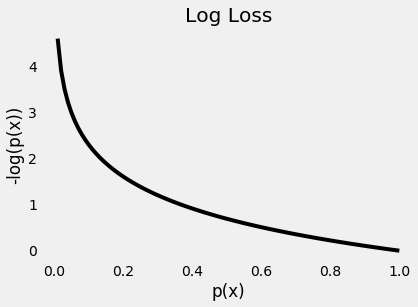
\includegraphics[scale=0.7]{img/binary_cross_neg_log}
	\caption{Negative log loss}
	\label{fig:binary_cross_neg_log}
\end{figure}

\subsection{Diving deeper}
\textbf{Entropy} is a measure of uncertainty associated with a given distribution $q(y)$.

$$H(q) = - \sum_{c=1}^C q(y_c) \cdot log(q(y_c))$$

Example with two classes (and $log$ base $2$):
\begin{itemize}
	\item
		All points from one class: $H(q) = - 1 \cdot log(1) = 0$ $\Rightarrow$ no uncertainty
	\item
		50:50 distribution: $H(q) = -log(0.5) = 1$ $\Rightarrow$ maximum uncertainty
\end{itemize}

So if we know the true distribution of a random variable, we can compute its entropy. But what if we don't know the true distribution? We can try to approximate the true distribution with some other distribution, namely $p(y)$.

\textbf{Cross-Entropy}. Let's assume our points follow this other distribution $p(y)$. But we know they are actually coming from the true distribution $q(y)$. If we compute entropy like this, we are actually computing the cross-entropy between both distributions:

$$H_p(q) = - \sum_{c=1}^C q(y_c) \cdot log(p(y_c))$$

If we, somewhat miraculously match $p(y)$ to $p(y)$ perfectly, the computed values for both cross-entropy and entropy will match as well. Since this is likely never happening, cross-entropy will have a BIGGER value than the entropy computed on the true distribution.

$$H_p(q) - H(q) \geq 0$$

The difference between cross-entropy and entropy is called \textbf{Kullback-Leibler Divergence} (KL Divergence), it is a measure of dissimilarity between two distributions:

$$D_{KL}(q||p) = H_p(q) - H(q) = \sum_{c=1}^C q(y_c) \cdot [log(q(y_c)) - log(p(y_c))]$$

This means that, the closer $p(y)$ gets to $q(y)$, the lower the divergence and, consequently, the cross-entropy, will be. So, we need to find a good $p(y)$ to use... but, this is what our classifier should do, isn't it? And indeed it does! It looks for the best possible $p(y)$, which is the one that minimizes the cross-entropy.

For our log loss we use $q(y_c) = 1/N_c$, so the number of samples we have for class $c$.

\section[Generative Adversarial Networks (GANs)]{Generative Adversarial Networks (GANs) \cite{goodfellow2016nips}}
\subsection{How do generative models work? How do GANs compare to others?}
To simplify the discussion somewhat, we will focus on generative models that
work via the principle of maximum likelihood. Not every generative model
uses maximum likelihood. Some generative models do not use maximum likelihood by default, but can be made to do so (GANs fall into this category). (Reminder MLE: $\theta^* = \argmax_{\theta} \prod_{i=1}^m p_{model}(x^{(i)}; \theta)$).

We can think of maximum likelihood estimation as minimizing the KL divergence between the data generating distribution and the model: $$\theta^* = \argmin_{\theta} D_{KL}(p_{data}(x)||p_{model}(x;\theta)).$$

If we were able to do this preciely, then if $p_{data}$ lies within the family of distributions $p_{model}(x; \theta)$, the model would recover $p_{data}$ exactly. In practice, we do not have access to $p_{data}$ itself, but only to a training set consiting of $m$ samples from $p_{data}$. We use these to define $\hat{p}_{data}$, an \textbf{empirical distribution} that places mass only on exactly those $m$ points, approximating $p_{data}$. Minimizing the KL divergence between $\hat{p}_{data}$ and $p_{model}$ is exactly equivalent to maximizing the log-likelihood of the training set.

\subsection{How do GANs work?}
The basic idea of GANs: set up game between two players. One of them is called \textbf{generator} and creates samples that are intended to come from the same distribution as the training data. The other player is the \textbf{discriminator} who examines samples to determine whether they are real or fake.

Formally, GANs are a structured probabilistic model containing latent variables $z$ and observed variables $x$. 


The two players in the game are represented by two functions, each of which is differentiable both with respect to its inputs and with respect to its parameters.
\begin{itemize}
	\item
		Discriminator: $D$ takes $x$ as input and uses $\theta^{(D)}$ as parameters
	\item
		Generator: $G$ takes $z$ as input and uses $\theta^{(G)}$ as parameters
\end{itemize}

Both players have cost functions that are defined in terms of both players’ parameters.
\begin{itemize}
	\item
		Discriminator: wishes to minimize $J^{(D)}(\theta^{(D)},\theta^{(G)})$ while controlling only $\theta^{(D)}$
	\item
		Generator: wishes to minimize $J^{(G)}(\theta^{(D)},\theta^{(G)})$ while controlling only $\theta^{(G)}$
\end{itemize}


Because each player's cost depends on the other player’s parameters, but each player cannot control the other player’s parameters, this scenario is most straightforward to describe as a game rather than as an optimization problem. The solution to an optimization problem is a (local) minimum, a point in parameter space where all neighboring points have greater or equal cost. The solution to a game is a Nash equilibrium. Here, we use the terminology of local differential Nash equilibria
(Ratliff et al., 2013). In this context, a Nash equilibrium is a tuple $(\theta^{(D)},\theta^{(G)})$ that is a local minimum of $J^{(D)}$ w.r.t $\theta^{(D)}$ and a local minimum of $J^{(G)}$ w.r.t $\theta^{(G)}$.

\textbf{The training process.} The training process consists of simultaneous SGD. On each step, two minibatches are sampled: a minibatch of $x$ values from the
dataset and a minibatch of $z$ values drawn from the model’s prior over latent
variables. Then two gradient steps are made simultaneously: one updating $\theta^{(D)}$ to reduce $J^{(D)}$ and one updating $\theta^{(G)}$ to reduce $J^{(G)}$. In both cases, it is possible to use the gradient-based optimization algorithm of your choice. Adam (Kingma and Ba, 2014) is usually a good choice.

\subsection{Cost functions}
Several different cost functions may be used within the GANs framework.

\subsubsection{The discriminators cost, $J^{(D)}$}
The cost used for the discriminator is:
$$J^{(D)}(\theta^{(D)},\theta^{(G)}) = -\frac{1}{2} \mathbb{E}_{x \sim{} p_{data}} log D(x) - \frac{1}{2} \mathbb{E}_z log(1 - D(G(z))).$$

This is just the standard cross-entropy cost that is minimized when training
a standard binary classifier with a sigmoid output. The only difference is that the classifier is trained on two minibatches of data; one coming from the dataset, where the label is 1 for all examples, and one coming from the generator, where the label is 0 for all examples. (\textit{Reminder:} $Entropy = H(q) = - \sum_{c=1}^C q(y_c) \cdot log(q(y_c)) = \mathbb{E}_{q\sim{}P} log(P(q)$) \cite{demys-tds}.

All versions of the GAN game encourage the discriminator to minimize this equation. In all cases, the discriminator has the same optimal strategy.

We see that by training the discriminator, we are able to obtain an estimate of the ratio $\frac{p_{data}(x)}{p_{model}(x)}$. Estimating this ratio enables us to compute a wide variety of divergences and their gradients. This is the key approximation technique that sets GANs apart from VACs and Boltzmann machines.
\subsubsection{Minimax}
A complete specification of the game requires that we specify a cost function also for the generator. From a game theoretic perspective D and G play the following two-player minimax game with value function $V(G, D)$:

$$min_G max_D V (D, G) = E_{x\sim{}p_{data}}(x)[log D(x)] + E_{z\sim{}p_z(z)}[log(1 - D(G(z)))].$$

The discriminator tries to maximize the objective function, therefore we can perform gradient ascent on the objective function. The generator tries to minimize the objective function, therefore we can perform gradient descent on the objective function. Look at figure \ref{fig:gan_minmax} for the algorithm.

\begin{figure}
	\centering
		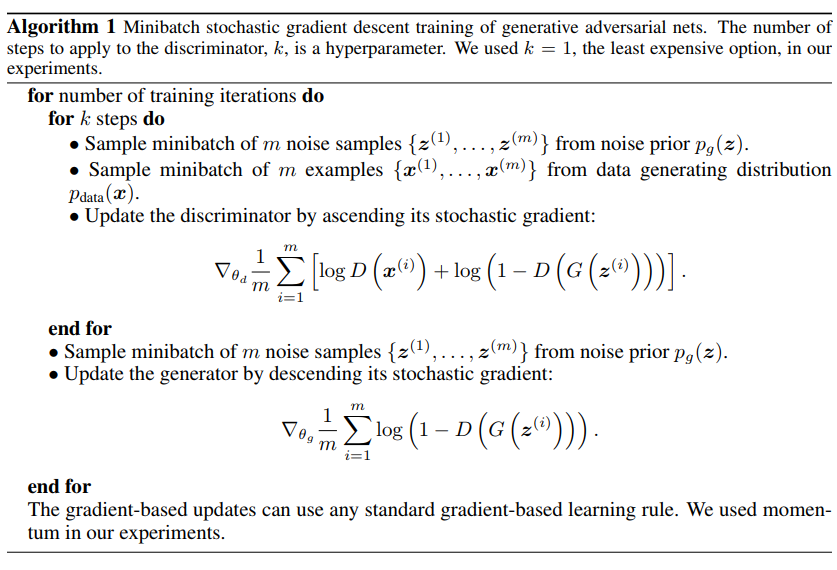
\includegraphics[scale=0.5]{img/gan_minmax}
	\caption{Minimax algorithm for GANs \cite{goodfellow2014generative}}
	\label{fig:gan_minmax}
\end{figure}

When applied, it is observed that optimizing the generator objective function does not work so well, this is because when the sample is generated it is likely to be classified as fake, the model would like to learn from the gradients but the gradients turn out to be relatively flat. This makes it difficult for the model to learn. Therefore, the generator objective function is changed to: $max_{G} \mathbb{E}_{z \sim{}p(z)} log(D(G(z)))$

Instead of minimizing the likelihood of the discriminator being correct, we maximize the likelihood of the discriminator being wrong. Therefore, we perform gradient ascent on the generator according to this objective function \cite{gansexpl-tds}.

\section{Deep Convolutional Generative Adversarial Networks (DCGAN)}
DCGANs are a family of architectures that resulted in stable training across a range of datasets and allowed for training higher
resolution and deeper generative models.

Architecture guidelines for stable Deep Convolutional GANs:
\begin{itemize}
	\item Replace any pooling layers with strided convolutions (discriminator) and fractional-strided convolutions (generator).
	\item Use batchnorm in both the generator and the discriminator. No batchnorm at generator output and discriminator input layer.
	\item Remove fully connected hidden layers for deeper architectures.
	\item Use ReLU activation in generator for all layers except for the output, which uses Tanh.
	\item Use LeakyReLU activation in the discriminator for all layers.
	\item Use Sigmoid at discriminator output, Tanh at generator.
\end{itemize}

More details:
\begin{itemize}
	\item
		Mini-batch SGD with mini-batch size of 128
	\item
		Weight-initialization from zero-centered normal distribution with standard deviation of 0.02
	\item
		Leaky-ReLU slope of 0.2
	\item
		Adam optimizer, learning rate of 0.0002, leaving momentum of 0.5
\end{itemize}

\begin{figure}
	\centering
		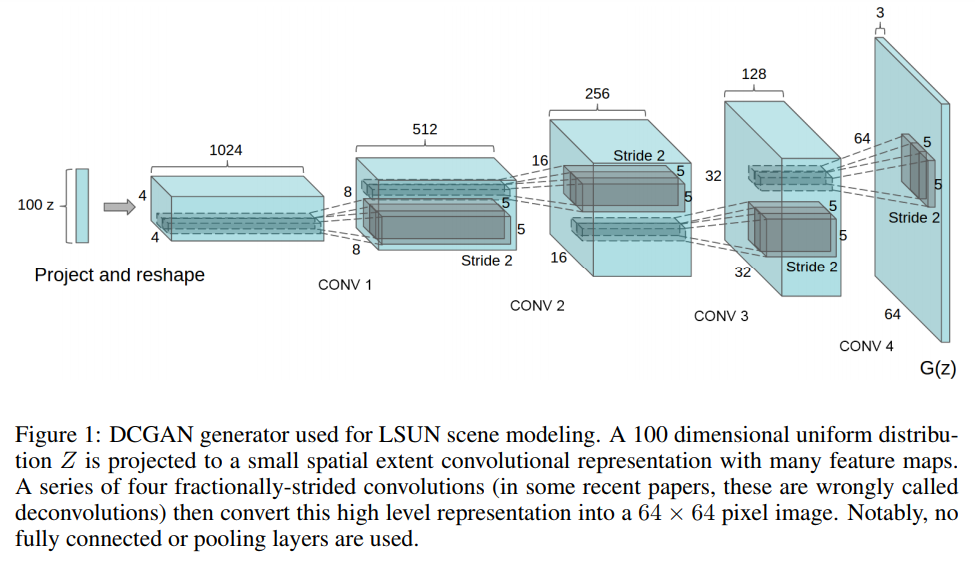
\includegraphics[scale=0.5]{img/dcgan_arch}
	\caption{}
	\label{fig:dcgan_arch}
\end{figure}

\section{Important formulas}
\subsection{Convolution}
$O:$ output size, $W:$ input size, $F:$ filter kernel size, $P:$ padding, $S:$ stride
\begin{itemize}
	\item
		Convolution: $O = \frac{W - F + 2P}{S} + 1$
	\item
		Transposed Convolution: $O = S(W-1) + F - 2P$
\end{itemize}

\newpage
\bibliographystyle{abbrv}
\bibliography{notes}
\end{document}